%Notes:Talk about what exactly a proxy server is
\chapter{Power Consumption Overhead for Proxy Services on Mobile Device Platforms}
\addcontentsline{toc}{section}{Introduction}
\section*{Introduction}
Current predictions by Cisco show that the amount of data that users consume has increased significantly and will continue to increase into the foreseeable future \cite{VNI14}. Previous studies show that the network interfaces of mobile devices consume much of the limited battery life \cite{Carroll:2010:APC:1855840.1855861}. Thus, heavy research efforts have been poured into studying the possibilities of energy efficient mobile data delivery. Some research avenues have middleware that acts as an on-device proxy service to realize benefits or enable new interaction paradigms, such as display networks \cite{6174992} or mobile content sharing \cite{Seeling:2014:OES:2671189.2671194},\cite{6692468}. To determine whether or not local proxy servers result in a large overhead in terms of power consumption and time delays, the measurement framework testbed described in Chapter \ref{ch:testbed} can be implemented to determine what kind of overheads can be expected from local proxy servers.

\addcontentsline{toc}{section}{Methodology and Metrics}
\section*{Methodology and Metrics}

\addcontentsline{toc}{subsection}{Measurement Setup}
\subsection*{Measurement Setup}
At the core of the setup, a Pandaboard ES mobile
software development platform is utilized, which features a Texas Instruments OMAP 4460 dual core ARM Cortex-A9 processor with
1 GB of DDR2 RAM, SMSC 10/100 Mbps Ethernet port, and
LS Research WLAN/Bluetooth wireless module, next to other
components. (Please refer to http://www.pandaboard.org for
more details. The open-source Android distribution
(version 4.1.2, ‘Jelly Bean’)  is used as the operating system software for the mobile device.
The overall measurement setup in can be seen in Figure \ref{fig:proxy_setup}. The
Pandaboard is powered by a BK Precision 1696 switchable
power supply, which features serial port access to read out
voltage and ampere values over time. The power
supply is connected to a Linux desktop computer serial port which timestamps
the values obtained over time to measure the power consumption
incurred by the Pandaboard. The Pandaboard is connected
through a 1 Gbps maximum speed Ethernet campus network,
which eliminates potential bottlenecks. For wireless measurements,
an externally connected WLAN antenna is utilized to
connect to the campus network through a dedicated WLAN access point, again eliminating bottlenecks for the
amounts of data considered throughout. It's also important to note
that a combination of input devices and an external monitor
were connected as well.
On the server side, a locally hosted virtual
machine next to Internet-routed web requests is utilized. The local server employs the Debian Linux distribution as its' operating system
with the Apache2 HTTP server and the popular Video Lan
Client (VLC) as media streaming application.A preencoded
video sequence of the popular open-source movie Tears
of Steel (see http://www.tearsofsteel.org for more information) is streamed utilizing HTML5 video streaming. The video-only sequence
was transcoded offline into a resolution of 864 × 480 at 24
frames per second in the Theora video codec and encapsulated
using the OGG container format, both commonly utilized for
HTTP video streaming “on the web” and suitable for mobile
playout. The resulting video bit stream has a duration of 12
minutes, 14 seconds and an average bit rate of 1.42 Mbps.
The bit rate in turn falls well within range of the network
bandwidth capacity.


\addcontentsline{toc}{subsection}{Mobile SOCKSv5 Proxy Server}
\subsection*{Mobile SOCKSv5 Proxy Server}
Several implementations of the SOCKSv5 standard 
exist to date \cite{rfc1928}, which allow utilization of a remotely hosted
standard-conforming SOCKSv5 proxy server (typically from
a desktop computer through an organizational server). Mobile
implementations, however, are less frequent. One example
of an implementation for the Android operating system is
the anonymity generating Orbot application (see http://www.
torproject.us for more details), which routes traffic into the
TOR network and contains “proxification” methods for applications
as well (i.e., transparently forcing the usage of the
proxy through, e.g., modifications of the iptables firewall). A basic Android service application was generated that is based on
the jSOCKS proxy server implementation \cite{kouzoubov2011}, which is open source
(entirely written in JAVA) and does not require any
privileges, such as root level system access. As the service is
executed within the Dalvik VM utilized on Android devices,
it incurs a minimal computational overhead when compared to
native applications. This approach, however, is commonplace
to allow broadest application compatibility and encouraged for
developers of the platform.

%Need to italicize as is done in paper
%Need to fix equations
\addcontentsline{toc}{subsection}{Performance Metrics}
\subsection*{Performance Metrics}
In the following, we briefly outline the metrics used to evaluate
the performance of either scheme. Initially, we capture
the reported voltage level v(tl) [V] and the current i(tl) [A]
as reported by the power supply and timestamped at time tl
on the connected desktop computer. We similarly calculate
the instant power consumption as p(tl) = v(tl) · i(tl) [W].
As the reported values are instantaneous snapshots in time
from l = 0 at t(l) = 0 (denoting the first measurement) to
l = L, which happened at t(l) = T (whereby T denotes
the last measurement), we calculate the time passed between
consecutive measurement instances as t(l) = tl − tl−1. To
determine the energy that was used in the l-th measurement
period, we calculate e(l) = t(l) · w(tl) [J]. We denote the
energy that was used in a measurement period up to t(l) as
\newline
\newline
Need to add in equations.
\newline

\begin{figure}
\centering
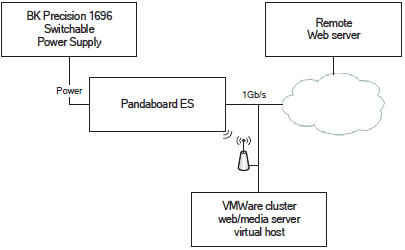
\includegraphics[scale=1,keepaspectratio]{proxy_setup}
\caption{Overview of the measurement setup}
\label{fig:proxy_setup}
\end{figure}

\addcontentsline{toc}{section}{Performance Evaluation For Web Requests}
\subsection*{Performance Evaluation For Web Request}
To perform a representative evaluation of frequent HTTP
web requests, web requests for Google’s home page were utilized.
The goal of this particular measurement scenario is to evaluate
the performance impact of frequent requests through the local
proxy server, which has to perform the additional connection
tasks each time a request is made. A direct
measurement application for Android was developed, which will request http://www.google.com without further resolving any
HTTP objects within. Individual requests are followed by a
sleep period of 2 seconds for both, direct requests and requests
through the mobile SOCKSv5 proxy service. As requests are
made without utilizing a browser, no caching is involved
client-side.

\addcontentsline{toc}{subsection}{Fixed Network}
\subsection*{Fixed Network}
In the fixed network scenario, the Pandaboard is connected
through wired Ethernet to the campus network while performing
the web requests. The requests typically coincide
with high power consumption levels, as illustrated in Figure \ref{fig:proxy_energy_cons_socks}
for an exemplary 100 web requests with both configurations.
We observe that both approaches exhibit an initial “spike”
behavior and an otherwise low level (with some general noise
due to overall device activities). There is no immediately
visible trend for the momentary power consumptions, as in
both approaches, there are several bursty periods of slightly
elevated consumptions on top of the actual web requests.
Next, we evaluate the total (compounded) energy consumption
that is observed when performing these requests for a
certain period of time. We illustrate 100 subsequent requests
directly and through the mobile proxy server in Figure \ref{fig:proxy_comp_energy_cons}.
Initially, it is observed that despite the short-term fluctuations,
there is a linear increase in the energy consumed
while using either approach. More significantly, there is no
immediately noticeable significant difference between the
approaches, which is indicated by the almost indistinguishable
values in the plot. Lastly, comparing the overhead between
the approaches numerically in Table \ref{tab:requests_summary}, where the
300 highest levels of energy consumption measured for periods
of placing 300 requests were analyzed. It's also notable that the direct approach
results in a higher average level of energy consumption (albeit
with a larger variability), whereas the proxy-based approach
yields a lower average and variability of energy usage values
determined. Overall, this results in an overhead of o =
−0.0563, which presents an initially counter-intuitive result.
(Differently worded, by utilizing the mobile proxy server
consuming additional CPU cycles, potential energy savings
of 5.6\% could be realized without requiring any additional
modifications.) Taking into account that partially significant
variability exists due to some outliers in the total duration
(as some measurement points can exhibit significant delays or
coincide with other unrelated system activities), both approaches are very similar.

\begin{figure}
\centering
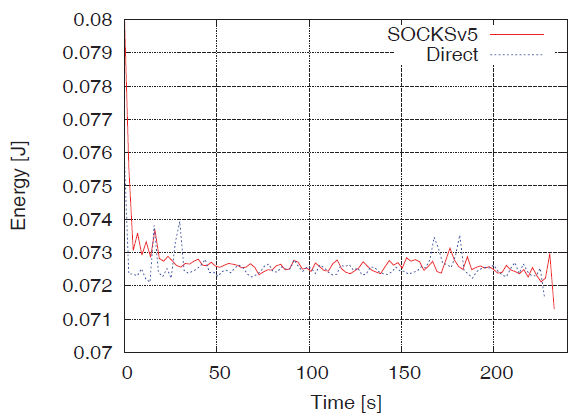
\includegraphics[scale=1,keepaspectratio]{proxy_energy_cons_socks}
\caption{Energy consumption while performing 100 web requests directly or through a mobile SOCKSv5 service, smoothed over time.}
\label{fig:proxy_energy_cons_socks}
\end{figure}

\begin{figure}
\centering
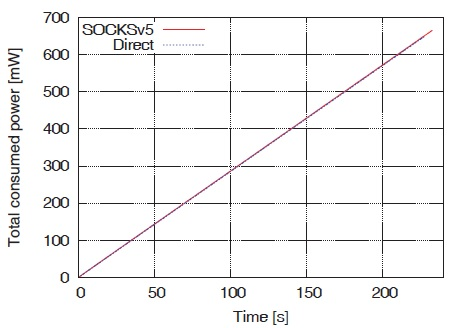
\includegraphics[scale=1,keepaspectratio]{proxy_comp_energy_cons}
\caption{Compounded energy consumption for performing 100 web requests directly or through a mobile SOCKSv5 service.}
\label{fig:proxy_comp_energy_cons}
\end{figure}

\begin{table}[h]
\begin{tabular}{|c|c|c|c|c|}
\hline
 Interface & Approach  & Average[J]  & Standard Deviation [J] & Confidence Interval (99 \%)  \\ \hline
 LAN & Direct & 0.0912 & 0.0139 & 0.0021 \\ \hline
 LAN & Proxy & 0.0860 & 0.0062 & 0.0009 \\ \hline
 WLAN & Direct & 0.0900 & 0.0125 & 0.0019 \\ \hline
 WLAN & Proxy & 0.0902 & 0.0089 & 0.0013 \\ \hline
\end{tabular}
\caption{Summary values for 300 direct and proxy-routed web requests over traditional ethernet and wireless LAN networks.}
\label{tab:requests_summary}
\end{table}

\addcontentsline{toc}{subsection}{Wireless Network}
\subsection*{Wireless Network}
Shifting the evaluation to HTTP requests made over the
wireless network interface, we present our results in Table \ref{tab:requests_summary}.
(We note that a graphical evaluation would yield results similar
to those presented in Figures \ref{fig:proxy_energy_cons_socks} and \ref{fig:proxy_comp_energy_cons}.) We initially note that
both approaches are very close with respect to their measured
average energy consumption, resulting standard deviations,
and narrow confidence intervals. \newline
Comparing these results with those obtained for the Ethernet
scenario, which outlines the base case without active wireless
communications overheads, we do not note a significant difference
in the average energy usage for the individual web
requests.

\addcontentsline{toc}{section}{Impact of Web Request Variations}
\subsection*{Impact of Web Request Variations}
Motivated by the closeness of requests, the next step is to more
closely evaluate the impact of the web request size over a
wireless LAN on the overall power consumption. To limit
the impact that external networks can have (such as different
delays), the direct performance comparison is performed within
the on-campus VM environment illustrated in Figure \ref{fig:proxy_setup}. A
dedicated virtual machine uses the Apache2 web server and
hosts a Python script that generates a requested number of
bytes, additionally eliminating potential caching impacts. 100 repeated measurements are performed for each different web request size and significant outliers are deleted.

\addcontentsline{toc}{subsection}{Power Consumption}
\subsection*{Power Consumption}

LEFT OFF FROM PAGE 44 IN PROXY PAPER